\documentclass{standalone}

\usepackage[euler-digits]{eulervm}

\usepackage{tikz}
\tikzset{every node/.style={circle,draw,minimum size=6mm,inner sep=0pt}}
\tikzset{t/.style={rectangle}}

\begin{document}
    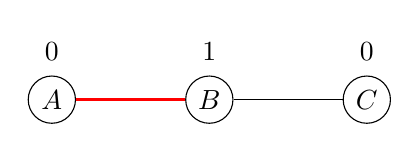
\begin{tikzpicture}[font=\sffamily]
      \node[label={$0$}] (A) at (0,0) {$A$}; 
      \node[label={$1$}] (B) at (2,0) {$B$}; 
      \node[label={$0$}] (C) at (4,0) {$C$}; 
      \draw[very thick,red] (A) -- (B);
      \draw (B) -- (C);
    \end{tikzpicture}
\end{document}
